\documentclass[12pt]{article}

\usepackage[utf8x]{inputenc}
\usepackage[L7x, T2A]{fontenc}
\usepackage[lithuanian]{babel}
\usepackage{vwcol}  
\usepackage{sectsty}
\usepackage{setspace}
\usepackage{fancyhdr}
\usepackage{graphicx}
\usepackage{ragged2e}
\usepackage{titlesec}
\usepackage{epsfig}
\usepackage{indentfirst}
\usepackage[top=2cm, bottom=2cm, left=3cm, right=1.5cm]{geometry}
\usepackage{makecell}
\usepackage{caption}
\usepackage{titlesec}

\usepackage{svg}

\makeatletter
\expandafter\let\csname L7x-cmd\endcsname\@changed@cmd
\makeatother

\addto\extraspolish{\fontencoding{L7x}\selectfont}
\addto\noextraspolish{\fontencoding{\encodingdefault}\selectfont}

\setlength\parindent{1cm}

\title{VILNIAUS UNIVERSITETAS \\
MATEMATIKOS IR INFORMATIKOS FAKULTETAS \\
PROGRAMŲ SISTEMŲ KATEDRA}
\author{}
\date{}

\pagestyle{fancy}
\fancyhead{}
\fancyfoot{}
\fancyfoot[R]{\thepage}
\renewcommand{\headrulewidth}{0pt}
\renewcommand{\baselinestretch}{1.5}
\renewcommand{\thesubsection}{\arabic{subsection}}
%\renewcommand{\thesubsubsection}{\thesubsection.\arabic{subsubsection}}

%\titleformat{\subsection}{\Large\bfseries}{\arabic{subsection}}{1em}{}
\titleformat{\subsubsection}{\large\bfseries}{\thesubsection.\arabic{subsubsection}}{1em}{}

\begin{document}
	\clearpage
	\maketitle
	\thispagestyle{empty}

	\bigbreak
	\bigbreak
	\bigbreak
	\bigbreak

	\begin{center}
		\begin{Large}
			\textbf{Transporto priemonių skelbimų aplikacija} \\
		\end{Large}
		\begin{large}
			\textbf{Application for Vehicle Advertisement} \\
		\end{large}
		Programų sistemų inžinerijos I laboratorinis darbas Nr. 2 \\

		\bigbreak
		\bigbreak
		\bigbreak
		\bigbreak
		\bigbreak
		\bigbreak
		\bigbreak
		\bigbreak
		\bigbreak

		\begin{tabular}{ll}
			Atliko:        & 2 kurso 5 grupės studentai \\
		               	   & Toma Burneikaitė \\
		               	   & Žygimantas Stongvilas \\
		                   & Mantas Jurčius \\
		                   & Rimvydas Meškauskas \\
			Darbo vadovas: & asist., dr., Vytautas Valaitis
		\end{tabular}

		\bigbreak
		\bigbreak
		\bigbreak
		\bigbreak
		\bigbreak
		\bigbreak
		\bigbreak
		\bigbreak
		\bigbreak

		Vilnius - 2018
	\end{center}
	\pagebreak
	
	\tableofcontents
	\pagebreak	
	
	\section*{Funkciniai reikalavimai}
	\addcontentsline{toc}{section}{Funkciniai reikalavimai}	
	
	\subsection{Bendri reikalavimai}
	\begin{enumerate}
		\item Įrenginys, kuriame naudojama programinė sistema, turi turėti prieigą prie interneto.
		\item Programinės įrangos įdiegimas turi būti laisvai prieinamas visiems norintiems ja naudotis.
		\item Vartotojas turės galimybę keisti savo asmeninius duomenis (vartotojo vardą ir slaptažodį).
		\item Skelbimai, pridėti prie mėgstamiausių sąrašo, bus saugomi vartotojo įrenginyje.
		\item Valiutų kursai nustatomi remiantis Lietuvos Banko duomenimis.
		\item Sistema vartotojui neprisijungus leis atlikti jos pagrindines funkcijas (skelbimų paieška).
		\item Sistema vartotojui prisijungus leis atlikti pagrindines (skelbimų paieška) ir papildomas funkcijas (mėgstamiausių sąrašas).
		\item Mėgstamiausių sąrašas atitinkamam vartotojui bus prieinamas tik jam ir niekam kitam.
		\item Sistema vartotojui leis iš bet kurio jos lango grįžti į pagrindinį langą.
	\end{enumerate}
	
	\subsection{Užsakovo reikalavimai}
	\begin{enumerate}
		\item Sistemos savininkas turi visas įmanomas sistemos teises (savas bei administratoriaus ir kliento).
		\item Sistemos savininkas gali paskirti naujus administratorius bei pašalinti esamus (suteikti arba atimti administratoriaus teises).
	\end{enumerate}	
	\pagebreak
	
	\subsection{Vartotojo reikalavimai}\label{Vartotojo_reikalavimai}
	Šiame skyriuje nagrinėjami vartotojui aktualūs reikalavimai sistemai „AutoINF“. Pateikiami vartotojo funkciniai reikalavimai, užduočių scenarijai bei jų plėtiniai.
	
	\begin{figure}[h]
		\begin{center}
			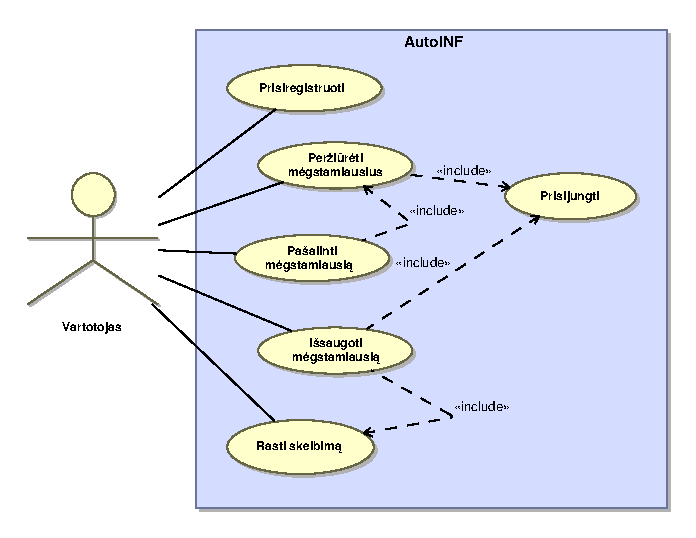
\includegraphics[width=0.7\textwidth]{TikslaiVartotojas.eps}
			\caption{Sistemos užduočių diagrama iš vartotojo perspektyvos\label{UseCaseUser}}
		\end{center}
	\end{figure}
	\pagebreak
	
	\subsubsection{Pagrindinio meniu reikalavimai ir scenarijus}
	\begin{enumerate}
		\item Pagrindiniame lange vartotojas, jei jis neprisijungęs, turi galimybę pasinaudoti sistemos funkcijomis: prisiregistruoti, prisijungti bei ieškoti skelbimų.
		
		\begin{center}
		\begin{tabular}{ | c | c | c | }
			\hline
			Žingsnis & Aktorius   & Veiklos apibūdinimas \\ \hline
			1        & Aplikacija & \makecell{Paprašo pasirinkti norimą veiksmą: \\ Prisiregistruoti \\ Prisijungti \\ Rasti skelbimą} \\ \hline
			2        & Vartotojas & Pasirenka veiksmą \\ \hline
			3        & Aplikacija & Įvykdo pasirinktą veiksmą \\ \hline
		\end{tabular}
		\captionof{table}{\leftskip = 2.8cm Pagrindinio lango scenarijus, kai vartotojas nėra prisijungęs\label{UserNotLoggedIn}}
		\end{center}
		
		\item Pagrindiniame lange vartotojas, jei jis prisijungęs, turi galimybę pasinaudoti šiomis sistemos funkcijomis: ieškoti skelbimų, peržiūrėti mėgstamiausius (registracijos mygtuko nebelieka).
		
		\begin{center}
		\begin{tabular}{ | c | c | c | }
			\hline
			Žingsnis & Aktorius   & Veiklos apibūdinimas \\ \hline
			1        & Aplikacija & \makecell{Paprašo pasirinkti norimą veiksmą: \\ Peržiūrėti mėgstamiausius \\ Pašalinti mėgstamiausią \\ Išsaugoti mėgstamiausią \\ Rasti skelbimą} \\ \hline
			2        & Vartotojas & Pasirenka veiksmą \\ \hline
			3        & Aplikacija & Įvykdo pasirinktą veiksmą \\ \hline
		\end{tabular}
		\captionof{table}{\leftskip = 2.82cm Pagrindinio lango scenarijus, kai vartotojas yra prisijungęs\label{UserLoggedIn}}
		\end{center}		
		
		\item Pagrindiniame lange turi būti pavaizduotas filtras, pagal kurį vartotojas gali ieškoti skelbimų.
	\end{enumerate}	
	\pagebreak
	
	\subsubsection{Vartotojo prisiregistravimo reikalavimai ir scenarijus}
	\begin{enumerate}
		\item Vartotojas, norintis prisiregistruoti, turi būtinai būti užpildęs registracijai reikiamus laukus. Jei paspaudus registracijos mygtuką kurie nors privalomi laukai yra palikti neužpildyti, tie laukai yra paryškinami raudonai ir šalia parodomas pranešimas, kad kai kurie registracijos laukai yra neužpildyti.
		
		\begin{center}
		\begin{tabular}{ | c | c | c | }
			\hline
			Žingsnis & Aktorius     & Veiklos apibūdinimas \\ \hline
			1        & Aplikacija   & Paprašo pasirinkti norimą veiksmą \\ \hline
			2        & Vartotojas   & Pasirenka registraciją \\ \hline
			3        & Aplikacija   & Atidaro registracijos langą \\ \hline
			4        & Vartotojas   & \makecell{Suveda prisiregistravimo duomenis ir \\ spaudžia mygtuką „Prisiregistruoti“} \\ \hline
			5        & Aplikacija   & \makecell{Patikrina duomenų formato teisingumą ir \\ siunčia duomenis į serverį} \\ \hline
			6        & Serveris     & Siunčia užklausą į duomenų bazę \\ \hline
			7        & Duomenų bazė & Perspėja serverį apie (ne)sėkmingą registraciją \\ \hline
			8        & Serveris     & Perspėja aplikaciją apie (ne)sėkmingą registraciją \\ \hline
			9        & Aplikacija   & \makecell{Parodo pranešimą apie registracijos (ne)sėkmingumą ir \\ perkrauna pagrindinį langą su prisijungusio vartotojo \\ interfeisu bei laukia, kol vartotojas atliks kitą veiksmą} \\ \hline
		\end{tabular}
		\captionof{table}{\leftskip = 5cm Vartotojo registracijos scenarijus\label{UserRegScen}}
		\end{center}	
		
		\item Registracijos laukai turi būti užpildyti reikiamu formatu (pvz., el. paštas -> test@mail.lt). Jei kurie nors laukai yra užpildyti neteisingu formatu, tai paspaudus registracijos mygtuką šitie laukai yra paryškinami raudonai ir šalia parodomas pranešimas, kad kai kurie laukai užpildyti neteisingai.
		\pagebreak
		\item Teisingai suvedus duomenis ir vartotojui paspaudus registracijos mygtuką sistema turi patikrinti, ar paskyra su tokiais duomenimis neegzistuoja, siekiant užtikrinti, kad nebūtų kelių paskyrų su tokiais pačiais el. paštais ar vartotojų vardais. Patikrinimui pasibaigus parodomas pranešimas apie registracijos (ne)sėkmingumą.	
		
		\begin{center}
		\begin{tabular}{ | c | c | c | }
			\hline
			Žingsnis & Sąlyga                                     & Veiklos apibūdinimas \\ \hline
			5a       & \makecell{Neteisingas \\ duomenų formatas} & \makecell{Klaidingai užpildyti laukai yra paryškinami raudonai \\ ir parodomas pranešimas, kad kai kurie \\ registracijos laukai yra užpildyti klaidingai} \\ \hline
			5b       & \makecell{Palikti \\ neužpildyti laukai}   & Neužpildyti laukai yra paryškinami raudonai \\ \hline
			7a       & \makecell{Duomenų bazėje \\ nepavyko išsaugoti \\ duomenų} & Parodomas pranešimas apie nesėkmingą registraciją \\ \hline
		\end{tabular}
		\captionof{table}{\leftskip = 4.1cm Vartotojo registracijos scenarijaus plėtiniai\label{UserRegScenExtra}}
		\end{center}
	\end{enumerate}	
	\pagebreak
	
	\subsubsection{Vartotojo prisijungimo reikalavimai ir scenarijus}
	\begin{enumerate}
		\item Vartotojui paspaudus prisijungimo mygtuką, sistema turi patikrinti, ar prisijungimo laukai užpildyti. Jei ne, vartotojui parodomas pranešimas, kad prisijungimo laukai palikti tušti.
		
		\begin{center}
		\begin{tabular}{ | c | c | c | }
			\hline
			Žingsnis & Aktorius     & Veiklos apibūdinimas \\ \hline
			1        & Vartotojas   & Pasirenka prisijungimo funkciją \\ \hline
			2        & Aplikacija   & Parodo prisijungimo langą \\ \hline
			3        & Vartotojas   & Suveda prisijungimo duomenis \\ \hline
			4        & Vartotojas   & Jungiasi su įvestais duomenimis \\ \hline
			5        & Aplikacija   & Siunčia užklausą į serverį \\ \hline
			6        & Serveris     & Siunčia užklausą į duomenų bazę \\ \hline
			7        & Duomenų bazė & Praneša serveriui apie sėkmingą prisijungimą \\ \hline
			8        & Serveris     & Praneša aplikacijai apie sėkmingą prisijungimą \\ \hline
			9        & Aplikacija   & \makecell{Parodo pagrindinį langą su papildomomis \\ prisijungusio vartotojo funkcijomis} \\ \hline
		\end{tabular}
		\captionof{table}{\leftskip = 5cm Vartotojo prisijungimo scenarijus\label{UserLogInScen}}
		\end{center}
		
		\item Jei prisijungimo laukai užpildyti, tai sistema patikrina, ar toks vartotojas egzistuoja. Jei vartotojo vardas ir slaptažodis įvesti teisingai, tai sistema perkrauną pagrindinį langą su prisijungusio vartotojo interfeisu. Jei vartotojo vardas ir slaptažodis įvesti neteisingai, tai vartotojui yra pranešama apie neteisingai suvestus duomenis.		
		
		\begin{center}
		\begin{tabular}{ | c | c | c | }
			\hline
			Žingsnis & Sąlyga                                     & Veiklos apibūdinimas \\ \hline
			4a       & \makecell{Vartotojas neužpildė \\ visų prisijungimo laukų} & Neužpildyti laukai yra paryškinami raudonai \\ \hline
			7a       & \makecell{Suvesti klaidingi \\ prisijungimo duomenys} & Parodomas pranešimas apie nesėkmingą prisijungimą \\ \hline
		\end{tabular}
		\captionof{table}{\leftskip = 4.1cm Vartotojo prisijungimo scenarijaus plėtiniai\label{UserLogInScenExtra}}
		\end{center}
		
	\end{enumerate}	
	\pagebreak
	
	\subsubsection{Vartotojo skelbimų ieškojimo reikalavimai ir scenarijus}
	\begin{enumerate}
		\item Vartotojui teisingai suvedus paieškos kriterijus ir paspaudus paieškos mygtuką, aplikacija turi ekrane parodyti visus rastus skelbimus, atitinkančius filtrą. Sistemai nesugebėjus rasti filtrą atitinkančių skelbimų, ekrane parodomas pranešimas, kad nepavyko rasti užklausą atitinkančių rezultatų.
		
		\begin{center}
		\begin{tabular}{ | c | c | c | }
			\hline
			Žingsnis & Aktorius     & Veiklos apibūdinimas \\ \hline
			1        & Vartotojas   & \makecell{Vartotojas įveda paieškos kriterijus ir \\ paspaudžia mygtuką „Ieškoti“} \\ \hline
			2        & Aplikacija   & Siunčia užklausą į serverį \\ \hline
			3        & Serveris     & Siunčia užklausą į paieškos modulį \\ \hline
			4        & Paieškos modulis & Grąžina serveriui rastus skelbimus \\ \hline
			5        & Serveris     & Grąžina aplikacijai rastus skelbimus  \\ \hline
			6        & Aplikacija   & Parodo rastų skelbimų sąrašą \\ \hline
			7        & Vartotojas   & Paspausžia ant skelbimo \\ \hline
			8        & Aplikacija   & Atidaro skelbimo langą \\ \hline
		\end{tabular}
		\captionof{table}{\leftskip = 4.3cm Vartotojo skelbimų ieškojimo scenarijus\label{UserSearchScen}}
		\end{center}		
		
		\begin{center}
		\begin{tabular}{ | c | c | c | }
			\hline
			Žingsnis & Sąlyga                                     & Veiklos apibūdinimas \\ \hline
			1a       & \makecell{Vartotojas nesuveda \\ paieškos kriterijų} & \makecell{Vartotojas įspėjamas, kad negalima \\ palikti neužpildytų privalomų laukų} \\ \hline
			5b       & Nerasta skelbimų                           & \makecell{Parodomas pranešimas, kad nėra skelbimų, \\ atitinkančių nurodytą filtrą, ir vartotojas yra \\ grąžinamas į pagrindinį langą } \\ \hline
			7a       & \makecell{Vartotojas nepaspaudžia \\ ant skelbimo} & \makecell{Aplikacija laukia, kol bus paspausta ant \\ skelbimo arba kol vartotojas ieškos naujų \\  skelbimų pagal kitą filtrą} \\ \hline
		\end{tabular}
		\captionof{table}{\leftskip = 3.3cm Vartotojo skelbimų ieškojimo scenarijaus plėtiniai\label{UserSearchScenExtra}}
		\end{center}		
		
	\end{enumerate}	
	
	\subsubsection{Vartotojo mėgstamiausių skelbimų peržiūrėjimo reikalavimai ir scenarijus}
	\begin{enumerate}
		\item Vartotojui paspaudus „Peržiūrėti mėgstamiausius“ mygtuką parodomas mėgstamiausių skelbimų sąrašas.
		
		\begin{center}
		\begin{tabular}{ | c | c | c | }
			\hline
			Žingsnis & Aktorius     & Veiklos apibūdinimas \\ \hline
			1        & Vartotojas   & Prisijungia prie sistemos \\ \hline
			2        & Aplikacija   & \makecell{Atidaro pagrindinį langą su papildomomis, \\ registruoto vartotojo, funkcijomis} \\ \hline
			3        & Vartotojas   & Pasirenka „Peržiūrėti mėgstamiausius“ funkciją \\ \hline
			4        & Aplikacija   & Siunčia užklausą į serverį \\ \hline
			5        & Serveris     & Siunčia užklausą į duomenų bazę \\ \hline
			6        & Duomenų bazė & Siunčia serveriui vartotojo mėgstamiausių skelbimų sąrašą \\ \hline
			7        & Serveris     & Siunčia aplikacijai vartotojo mėgstamiausių skelbimų sąrašą \\ \hline
			8        & Aplikacija   & \makecell{Atidaro naują langą su vartotojo išsaugotais \\ jo mėgstamiausiais skelbimais } \\ \hline
		\end{tabular}
		\captionof{table}{\leftskip = 3.3cm Vartotojo mėgstamiausių skelbimų peržiūrėjimo scenarijus\label{UserViewFavScen}}
		\end{center}		
	\end{enumerate}	
	\pagebreak
	
	\subsubsection{Vartotojo mėgstamiausio skelbimo pašalinimo reikalavimai ir scenarijus}
	\begin{enumerate}
		\item Vartotojui paspaudus mygtuką „Trinti“ aplikacija išmeta papildomą sisteminį langą, kuriame klausiama vartotojo, ar jis tikrai nori panaikinti šį skelbimą iš savo mėgstamiausių sąrašo. Paspaudus „Taip“ skelbimas sėkmingai panaikinamas iš mėgstamiausių sąrašo. 
		
		\begin{center}
		\begin{tabular}{ | c | c | c | }
			\hline
			Žingsnis & Aktorius       & Veiklos apibūdinimas \\ \hline
			1        & Vartotojas     & Pasirenka mėgstamiausių skelbimų langą \\ \hline
			2        & Aplikacija     & \makecell{Atidaro mėgstamiausių skelbimų langą ir \\ laukia tolesnių vartotojo veiksmų} \\ \hline
			3        & Vartotojas     & Pasirenka skelbimo šalinimą \\ \hline
			4        & Aplikacija     & Siunčia užklausą į serverį \\ \hline
			5        & Serveris       & Siunčia užklausą į duomenų bazę  \\ \hline
			6        & Duomenų bazė   & \makecell{Pašalina mėgstamiausią skelbimą iš duomenų bazės \\ ir grąžina pranešimą apie sėkmingai pašalintą skelbimą} \\ \hline
			7        & Serveris       & \makecell{Grąžina pranešimą apie sėkmingai \\ pašalintą mėgstamiausią skelbimą} \\ \hline
			8        & Aplikacija     & Atnaujina mėgstamiausių skelbimų sąrašą \\ \hline
		\end{tabular}
		\captionof{table}{\leftskip = 3cm Vartotojo mėgstamiausio skelbimo pašalinimo scenarijus\label{UserRemoveAdScen}}
		\end{center}	
		
		\begin{center}
		\begin{tabular}{ | c | c | c | }
			\hline
			Žingsnis & Sąlyga                                     & Veiklos apibūdinimas \\ \hline
			6a       & \makecell{Nepavyko pašalinti \\ skelbimo iš \\ duomenų bazės} & \makecell{Grąžina pranešimą apie nesėkmingą \\ skelbimo pašalinimą iš duomenų bazės} \\ \hline
		\end{tabular}
		\captionof{table}{\leftskip = 2.2cm Vartotojo mėgstamiausio skelbimo pašalinimo scenarijaus plėtiniai\label{UserRemoveAdExtra}}
		\end{center}
	\end{enumerate}	
	\pagebreak	
	
	\subsubsection{Vartotojo mėgstamiausio skelbimo išsaugojimo reikalavimai ir scenarijus}
	\begin{enumerate}
		\item Vartotojui paspaudus skelbimo išsaugojimo mygtuką, skelbimas yra įtraukiamas į vartotojo mėgstamiausių skelbimų sąrašą ir sistema informuoja vartotoją apie sėkmingai atliktą veiksmą.
		
		\begin{center}
		\begin{tabular}{ | c | c | c | }
			\hline
			Žingsnis & Aktorius         & Veiklos apibūdinimas \\ \hline
			1        & Vartotojas       & Vykdo skelbimų paiešką \\ \hline
			2        & Aplikacija       & Siunčia užklausą į serverį \\ \hline
			3        & Serveris         & Siunčia užklausą į paieškos modulį \\ \hline
			4        & Paieškos modulis & Grąžina serveriui paieškos rezultatus \\ \hline
			5        & Serveris         & Grąžina aplikacijai paieškos rezultatus  \\ \hline
			6        & Aplikacija       & Parodo rastų skelbimų sąrašą \\ \hline
			7        & Vartotojas       & Prideda norimą skelbimą prie mėgstamiausių \\ \hline
			8        & Aplikacija       & Siunčia užklausą į serverį \\ \hline
			9        & Serveris         & Siunčia užklausą į duomenų bazę \\ \hline
			10       & Duomenų bazė     & \makecell{Išsaugo skelbimą mėgstamiausių sąraše ir \\ praneša serveriui apie sėkmingą skelbimo išsaugojimą} \\ \hline
			11       & Serveris         & Praneša aplikacijai apie sėkmingą skelbimo išsaugojimą \\ \hline
			12       & Aplikacija       & Praneša apie sėkmingą skelbimo išsaugojimą \\ \hline
		\end{tabular}
		\captionof{table}{\leftskip = 3cm Vartotojo mėgstamiausio skelbimo išsaugojimo scenarijus\label{UserSaveAdScen}}
		\end{center}	
		\pagebreak		
	\end{enumerate}	
	\pagebreak
	
	\subsection{Administratoriaus reikalavimai}
	Šiame skyriuje nagrinėjami administratoriui aktualūs reikalavimai sistemai „AutoINF“. Pateikiami administratoriaus funkciniai reikalavimai, užduočių scenarijai bei jų plėtiniai.
	
	\begin{figure}[h]
		\begin{center}
			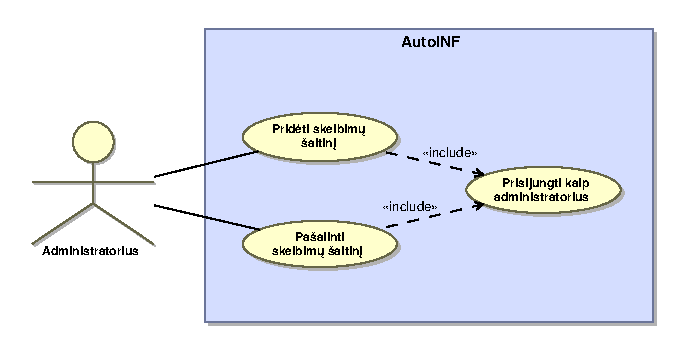
\includegraphics[width=0.7\textwidth]{TikslaiAdministratorius.eps}
			\caption{Sistemos užduočių diagrama iš administratoriaus perspektyvos\label{UseCaseAdmin}}
		\end{center}
	\end{figure}
	\pagebreak
	
	\subsubsection{Administratoriaus prisijungimo reikalavimai ir scenarijus}
	\begin{enumerate}
		\item Sistema užtikrina, kad prisijungimo duomenys suvesti teisingai.
		\item Prisijungus yra perkraunamas pagrindinis langas su prisijungusio administratoriaus interfeisu. 
		
		\begin{center}
		\begin{tabular}{ | c | c | c | }
			\hline
			Žingsnis & Aktorius         & Veiklos apibūdinimas \\ \hline
			1        & Aplikacija       & \makecell{Aplikacija paprašo pasirinkti norimą veiksmą: \\ Pridėti skelbimų šaltinį \\ Pašalinti skelbimų šaltinį} \\ \hline
			2        & Administratorius & Administratorius pasirenka veiksmą \\ \hline
			3        & Aplikacija       & Aplikacija įvykdo pasirinktą veiksmą \\ \hline
		\end{tabular}
		\captionof{table}{\leftskip = 2.2cm Pagrindinio lango scenarijus, kai administratorius yra prisijungęs\label{UserNotLoggedIn}}
		\end{center}	
		
		\begin{center}
		\begin{tabular}{ | c | c | c | }
			\hline
			Žingsnis & Aktorius         & Veiklos apibūdinimas \\ \hline
			1        & Administratorius & Prisijungia \\ \hline
			2        & Aplikacija       & \makecell{Atidaro pagrindinį langą su administratoriaus interfeisu ir \\ laukia, kol administratorius atliks kokį veiksmą} \\ \hline
			3        & Administratorius & Pasirenka peržiūrėti skelbimų šaltinius \\ \hline
			4        & Aplikacija       & Siunčia užklausą į serverį \\ \hline
			5        & Serveris         & Siunčia užklausą į duomenų bazę \\ \hline
			6        & Duomenų bazė     & Grąžina skelbimų šaltinių sąrašą į serverį \\ \hline
			7        & Serveris         & Grąžina skelbimų šaltinių sąrašą į aplikaciją \\ \hline
			8        & Aplikacija       & Parodo skelbimų šaltinių sąrašą \\ \hline
		\end{tabular}
		\captionof{table}{\leftskip = 3.2cm Administratoriaus peržiūrėti skelbimų šaltinius scenarijus\label{AdminViewSourcesScen}}
		\end{center}	
		
		\begin{center}
		\begin{tabular}{ | c | c | c | }
			\hline
			Žingsnis & Sąlyga         & Veiklos apibūdinimas \\ \hline
			6a       & \makecell{Duomenų bazėje \\ nėra šaltinių} & \makecell{Duomenų bazė grąžina pranešimą, kad \\ skelbimų šaltinių nėra} \\ \hline
		\end{tabular}
		\captionof{table}{\leftskip = 3cm Administratoriaus peržiūrėti skelbimų šaltinius scenarijaus plėtiniai\label{AdminViewSourcesScenExtra}}
		\end{center}	
		
	\end{enumerate}	
	
	\subsubsection{Administratoriaus skelbimų šaltinio pridėjimo reikalavimai ir scenarijus}
	\begin{enumerate}
		\item Pasirinkęs skelbimų šaltinių pridėjimo funkciją administratorius gali pridėti kokios nors tai svetainės URL ir ši svetainė pridedama į skelbimų šaltinių sąrašą.
		
		begin{enumerate}
		\item Pasirinkęs skelbimų šaltinio šalinimo funkciją administratorius gali pašalinti pasirinktą šaltinį iš sistemos duomenų bazės. 
		
		\begin{center}
		\begin{tabular}{ | c | c | c | }
			\hline
			Žingsnis & Aktorius         & Veiklos apibūdinimas \\ \hline
			1        & Administratorius & Pasirenka skelbimų šaltinių peržiūros funkciją \\ \hline
			2        & Aplikacija       & Parodo skelbimų šaltinius \\ \hline
			3        & Administratorius & \makecell{Suveda naujo skelbimų šaltinio duomenis ir \\ spaudžia mygtuką „Pridėti šaltinį“ } \\ \hline
			4        & Aplikacija       & Siunčia užklausą į serverį \\ \hline
			5        & Serveris         & Siunčia užklausą į duomenų bazę \\ \hline
			6        & Duomenų bazė     & \makecell{Prideda naują skelbimų šaltinį ir praneša \\ serveriui apie sėkmingą skelbimų šaltinio pridėjimą} \\ \hline
			7        & Serveris         & \makecell{Praneša aplikacijai apie sėkmingą skelbimų \\ šaltinio pridėjimą} \\ \hline
			8        & Aplikacija       & Atnaujina skelbimų šaltinių sąrašą \\ \hline
		\end{tabular}
		\captionof{table}{\leftskip = 3.2cm Administratoriaus skelbimų šaltinio pridėjimo scenarijus\label{AdminAddSourceScen}}
		\end{center}	
		
		\begin{center}
		\begin{tabular}{ | c | c | c | }
			\hline
			Žingsnis & Sąlyga         & Veiklos apibūdinimas \\ \hline
			6a       & \makecell{Nepavyksta \\ pridėti šaltinio} & \makecell{Duomenų bazė grąžina pranešimą apie \\ nesėkmingą skelbimų šaltinio pridėjimą} \\ \hline
		\end{tabular}
		\captionof{table}{\leftskip = 3cm Administratoriaus skelbimų šaltinio pridėjimo scenarijaus plėtiniai\label{AdminAddSourceScenExtra}}
		\end{center}		
	\end{enumerate}	
	\pagebreak
	
	\subsubsection{Administratoriaus skelbimų šaltinio pašalinimo reikalavimai ir scenarijus}
	\begin{enumerate}
		\item Pasirinkęs skelbimų šaltinio šalinimo funkciją administratorius gali pašalinti pasirinktą šaltinį iš sistemos duomenų bazės. 
		
		\begin{center}
		\begin{tabular}{ | c | c | c | }
			\hline
			Žingsnis & Aktorius         & Veiklos apibūdinimas \\ \hline
			1        & Administratorius & \makecell{Pasirenka skelbimų šaltinių peržiūros \\ funkciją ir pasirenka šaltinio šalinimą} \\ \hline
			2        & Aplikacija       & Siunčia užklausą serveriui \\ \hline
			3        & Serveris         & Siunčia užklausą duomenų bazei \\ \hline
			4        & Duomenų bazė     & \makecell{Pašalina skelbimų šaltinį ir siunčia pranešimą \\ serveriui apie sėkmingai pašalintą skelbimų šaltinį} \\ \hline
			5        & Serveris         & \makecell{Siunčia pranešimą aplikacijai apie \\ sėkmingai pašalintą skelbimų sąrašą} \\ \hline
			6        & Aplikacija       & \makecell{Atnaujina skelbimų sąrašą ir laukia \\ tolimesnių administratoriaus veiksmų} \\ \hline
		\end{tabular}
		\captionof{table}{\leftskip = 3.2cm Administratoriaus skelbimų šaltinio šalinimo scenarijus\label{AdminRemoveSourceScen}}
		\end{center}	
		
		\begin{center}
		\begin{tabular}{ | c | c | c | }
			\hline
			Žingsnis & Sąlyga         & Veiklos apibūdinimas \\ \hline
			4a       & \makecell{Nepavyksta \\ pašalinti šaltinio} & \makecell{Duomenų bazė grąžina pranešimą apie \\ nesėkmingą skelbimų šaltinio pašalinimą} \\ \hline
		\end{tabular}
		\captionof{table}{\leftskip = 3cm Administratoriaus skelbimų šaltinio šalinimo scenarijaus plėtiniai\label{AdminRemoveSourceScenExtra}}
		\end{center}	
		
		
	\end{enumerate}
	\pagebreak
	
	\section*{Nefunkciniai reikalavimai}
	\addcontentsline{toc}{section}{Nefunkciniai reikalavimai}
	\setcounter{subsection}{0}
	
	\subsection{Vidinių interfeisų reikalavimai}
	\begin{enumerate}
		\item Sistema turi būti suprogramuota Java programavimo kalba.
		\item Sistema bus sukompiliuota laisvai platinamu standartiniu Java kompiliarotiumi.
		\item Sistema veiks Android aplinkoje, versijos pasirinkimas paliekamas programuotojų nuožiūrai.
		\item Programavimo aplinkos pasirinkimas paliekamas programuotojų nuožiūrai.
		\item Duomenims saugoti naudojama PostgreSQL duomenų bazė.
	\end{enumerate}	
	
	\subsection{Veikimo reikalavimai}
	Šiame skyriuje aprašomi sistemos veikimo reikalavimai.
	
	\subsubsection{Tikslumo reikalavimai}
	\begin{enumerate}
		\item Skelbimo kaina atvaizduojama double formatu 2 skačių po kablelio tikslumu ir nėra apvalinama.
		\item Duomenys apie valiutą saugomi double formatu. Skaičių kiekis po kablelio neribojamas.
	\end{enumerate}	
	
	\subsubsection{Patikimumo reikalavimai}
	\begin{enumerate}
		\item Įvykus kokiam nors sistemos sutrikimui, sistema turi perkelti vartotoją į prieš tai atliktą žingsnį.
		\item Įvykus sutrikimui sistema neatskleidžia vidinių sutrikimo priežasčių vartotojui (nebent sutrikimas įvyko dėl jo kaltės). Visus sistemos lūžius ir to priežastis sistema saugo duomenų bazėje, prieinamoje tik savininkui ir administratoriui.
		\item Skelbimas vartotojo mėgstamiausiųjų sąraše atsiranda tik tada, kai jis pridedamas į duomenų bazę.
		\item Sistema nebus galima naudotis, kai bus atnaujinama sistemos duomenų bazė.
	\end{enumerate}	
	
	\subsubsection{Robastiškumo reikalavimai}
	\begin{enumerate}
		\item Visos klaidos yra saugomos sistemos duomenų bazėje, klaidų registre.
		\item Įvykus nedideliam sutrikimui (pvz., dingsta ryšys su duomenų baze; neatsako skelbimų puslapiai) sistema kartoja paskutinį veiksmą 30 s. Neatsistačius funkcionalumui sistema išsaugo klaidos priežastį duomenų bazėje, atsiprašo vartotojo už nepatogumus ir prašo vartotojo pabandyti naudotis sistema vėliau.
		\item Įvykus rimtam sutrikimui (pvz., atnaujintas skelbimų puslapio HTML kodas; pasikeičia skelbimų nuskaitymo būdas, todėl nebeįmanoma gauti skelbimų informacijos, nors puslapis ir atsako), sistema turi gebėti išimti puslapį iš pasirinkimo galimybių ir užregistruoti veiksmą duomenų bazėje.
		\item Po sistemos sutrikimo tikėtinas atsistatymo laikas yra laikas, reikalingas sistemos perkrovimui.
		\item Sutrikus infrastruktūrai (pvz., duomenų bazei) sistema pradės veikti iš karto, kai infrastruktūra bus sutvarkyta.
	\end{enumerate}	
	
	\subsubsection{Našumo reikalavimai}
	\begin{enumerate}
		\item Sistema iš karto turi pranešti vartotojui, kad priėmė paieškos duomenis ir kad paieška yra vykdoma.
		\item Sistema turėtų parodyti pirmąjį užklausos puslapį ne lėčiau kaip per 10 s.
		\item Sistema į vartotojo įvestį turi sureguoti ne lėčiau kaip per 0,5 s.
		\item Užklausų skaičius, kurį maksimaliai be vėlavimo gali atlikti serveris, yra 10 000 per sekundę (nebent sistemos savininko infrastruktūra nėra pakankamai pajėgi).
	\end{enumerate}
	
	\subsection{Interfeiso reikalavimai}	
	\begin{enumerate}
		\item Originali valiuta automatiškai konvertuojama į eurus, bet vartotojas gali pasirinkti, kurią valiutą iš pagrindinių (pagrindinės valiutos pasirenkamos programuotojų atžvilgiu, bet nemažiau kaip 3, iš kurių viena - euras) rodyti.
		\item\label{MainWindowDisplayReq} Pagrindinis langas, kuris atvaizduojamas tik įjungus programą, yra paieškos langas. 
		\item\label{AdParts} Visi skelbimai sąraše atvaizduojami formatu, kurio pagrindinės dalys yra:
		
		\begin{enumerate}
			\item[\ref{AdParts}.1.] Pagrindinė skelbimo nuotrauka,
			\item[\ref{AdParts}.2.] Automobilio markė,
			\item[\ref{AdParts}.3.] Automobilio modelis,
			\item[\ref{AdParts}.4.] Kuro tipas,
			\item[\ref{AdParts}.5.] Variklio litražas,
			\item[\ref{AdParts}.6.] Kėbulo tipas,
			\item[\ref{AdParts}.7.] Kaina.
		\end{enumerate}
		
		\item Paieškos lange turi būti leidžiama pasirinkti skelbimo pagrindinių dalių paieškos filtrus, tačiau galima ir platesnė paieška.
		\item Viename paieškos rezultatų lange maksimaliai gali būti 20 skelbimų.
		\item Sistemoje turi būti įdiegta galimybė bet kuriame jos etape grįžti į pagrindinį paieškos langą ir, jei vartotojas yra prisijungęs, į mėgstamiausių skelbimų sąrašo langą (jei vartotojas nėra prisijungęs - į prisijungimo langą). Siūlomas sprendimas - įrankių juosta viršuje visų langų.
	\end{enumerate}	
	
	\subsection{Ergonominiai reikalavimai}		
	\begin{enumerate}
		\item Šriftų dydis pagrindiniame lange ne mažesnis nei 20 pt, skelbimo formate - ne mažesnis nei 10 pt.
		\item Tarpai tarp eilučių turi būti tokie, kad eilutės nesiliestų viena su kita.
		\item Atsižvelgiant į interfeiso reikalavimų \ref{MainWindowDisplayReq} punktą vartotojui nedetalizavus paieškos pagrindiniam sistemos veiksmui (paieškai) atlikti
užtenka 1 veiksmo.
		\item Sistema neturi būti pritaikyta neįgaliesiems.
	\end{enumerate}
	
\end{document}